\documentclass[hidelinks,english]{article}

\usepackage{graphicx}
\usepackage{grffile}
\usepackage[T1]{fontenc}
\usepackage{babel}
\usepackage{wrapfig}
\usepackage{hyperref}

\date{\today}

\graphicspath{{Pictures/}}
\begin{document}	
	\begin{titlepage}
		\pagenumbering{gobble}
		\begin{figure}[!t]
			
\includegraphics[width=\linewidth]{up_logo.png}
		\end{figure}
		\vspace*{\stretch{1.2}}
		\begin{center}
			\huge{Architectural and Functional Requirements\\}
			\huge{Mindmap PIM}\\
			\large{Client: IMINISYS}\\
			\vspace{10mm}
			\huge{Team: A-Cube-N}\\
		\end{center}
		\begin{center}
			\begin{tabular}{ c c c }
				Grobler, Arno & Lochner, Amy & Maree, Armand \\
				\texttt{14011396} & \texttt{14038600}& \texttt{12017800} \\				
			\end{tabular}
		\end{center}
		\begin{center}
			Department of Computer Science, University of Pretoria
		\end{center}
		\vspace*{\stretch{2.0}}
	\end{titlepage}
	\newpage
	\tableofcontents
	\newpage
	\pagenumbering{arabic}
	
	\section{Introduction} 
		\paragraph\indent
		People of this day and age often make use of many technologies and platforms for the purpose of staying in contact with people, sharing moments with friends, communicating with people and organising their day-to-day lives. Generally all the above tasks of a person in the 21st century are done on different platforms for example Facebook, Email and Google Calendar. This project serves to provide a single platform where the information of its users from various platforms are organised into topics. 
	
	
	\section{Vision}
		\paragraph\indent
		The vision of this project is to create an application which extracts data from various existing platforms such as Gmail and Facebook. The application will make use of a natural language processor to extract data, determine the general topic of the data then integrate this new information into the interactive mind map. The hope is that this will simplify the user's life by only needing one application to 'monitor' all other platforms on which they might have an account and manage the information of those platforms from our application. The mind map will work in a similar fashion as our minds work. Where the exploration of one topic may lead to the exploration of another topic that is related to the user. Hence the "mind" map, it is a map of your mind visualized by the topics that come up in your life.
	
	\section{Background}
		\paragraph\indent
		We got elected for this project by including it as one of our top 3 choices for the projects that we wanted to do most. Once we were chosen for this project, we began to learn more about what the client expected from us.

		\subsection{Future business/research opportunities}
			\paragraph\indent
			The Mind Mapped PIM project provides an opportunity for us to create something that helps to simplify the user's life. It will do this by organizing all relevant information into one system. It can also help the user to plan out their daily and weekly schedules which can lead to reduced stress on the user.
		
		\subsection{The Client's Problem}
			\paragraph\indent
			The client wants to have a way of displaying all relevant information in one place in the form of a mind map. This will help to organize general life events such as meetings. This information will come from different sources and enables the user to see all relevant information without having to go to each source individually. A key aspect is that Mind Map PIM attempts to dig through the clutter contained in other PIMs and only display things the user might want to see.
		
	\section{Important Terminology}
		\begin{itemize}
			\item \textbf{Unclutter} Commercial name for the application.
			\item \textbf{Bubble} A single node in the mind map.
			\item \textbf{Bubble Map} The mind map that is presented to the user.
			\item \textbf{PIM} Personal Information Manager such as Google Calendar and social media platforms like Facebook.
			\item \textbf{Data Source} It refers to the source where user data is retrieved from.
			\item \textbf{Poller} The service which will constantly ask a data source for new information and then send new information to the processing service.
		\end{itemize}	
	
	\section{Architecture Requirements}
		\subsection{Access Channel Requirements}
    		\subsubsection{Human Access Channels}
    			\paragraph\indent
                Users  will access the system through a website. It should be available to anyone wishing to sign up through any browser i.e. Chrome, Mozilla Firefox, Internet Explorer, Safari and Edge provided the user has a Gmail or Facebook account with which to sign up. It is our intention to ensure that the website will be under strict standards-compliance, that is, having the website comply with the World Wide Web Consortium (W3C) (W3C, 2016) so that the website will run on every browser exactly the same. The website should be mobile friendly as to be able to scale down to a phone screen size and still be usable and interactive. Offline capabilities for users who have already used the service before would be a nice-to-have feature.
                
            \subsubsection{System Access Channels}
            	\paragraph\indent
                Websocket based web services will be used as the primary means of communication between the interface and the front end application. This is due to the bi-directional communication that it offers.
                
                A technology known as RabbitMQ will be used to allow communication between our multiple back end applications such as the polling applications, business logic application and the database application.
		
		\subsection{Quality Requirements}
			\paragraph\indent
	        The following quality requirements have been placed in order of priority.
	        
            \subsubsection{Performance}
            	\paragraph\indent
                Performance has the highest priority since this system has to be real time. Any new information that is updated on the respective websites and email clients should, in the least amount of time possible, update the mind map too. Thus the backend processing and persistence of new information should happen rapidly.
                
                \paragraph\indent
                Performance in terms of front-end should also be addressed. The system is a fully graphic website and thus should give the user the most fluid and smooth experience. To implement a fast interactive system technologies such as HTML canvas can be used to render the graph with smooth user interaction.
                
            \subsubsection{Usability}
            	\paragraph\indent
                Usability is the second highest priority as the system is fully graphic in terms of what the end user will use. The system needs to have a very good User Experience (UX) and must be completely user friendly so it is not difficult to use.
                
            \subsubsection{Reliability}
            	\paragraph\indent
                The system needs to be reliable, since it has to provide information in real time. This cannot happen if the system is constantly down. Thus hot reloading will be used to update static files like JavaScript and HTML. Since RabbitMQ stores messages while the system is running, it is possible to reboot backend services while the system is running. Any pending messages will be processed as soon as the service is fully up and running again.
                
                \paragraph\indent
                Reliability also refers to providing accuracy, and such needs to be implemented to provide the correct information to the right bubbles.
                
            \subsubsection{Scalability}
                \paragraph\indent
                This system needs to be highly scalable. The large number of users should not affect the system's performance. Thus a queue messaging broker (RabbitMQ) will be used to handle a large number of requests. This will pervent backend processes responsible for data processing to be flooded with requests.
                
            \subsubsection{Flexibility}
            	\paragraph\indent
                The system must be flexible in terms of the plugablity of polling services. A new polling service for a new PIM should be able to integrate with no change of the rest to the system. The system also should be able to function with any combination of PIMs that a user selects.

            \subsubsection{Security}
            	\paragraph\indent
                The system should be very secure since it is using private information that belongs solely to that user. Private information such as emails and photos isn't something that users would like other people seeing. Thus a secure login process has to be implemented. Since Google and Facebook have both good log in systems, we will use that to log in to the system by using the OAUTH2 protocol.
                
            \subsubsection{Integrability}
            	\paragraph\indent
                The system should be developed in such a way that new polling services can easily integrate with the already implemented system.

		\subsection{Integration Requirements}
			\begin{enumerate}
		        \item \textbf{HTTP:}\\
		            This is the main protocol for all websites and will be the interface for the user to easily navigate the system.
		        \item \textbf{REST:}\\
		            REST will be implemented as the communication protocol between backend services. It is simple to implement and integrates well with systems already operational. REST will be useful in this case since the system does not care from which poller information comes from.
		        \item \textbf{TCP:}\\
		            This protocol will be needed to establish network connections between the user's computers and the system servers. These data streams can then be exchanged between the connected machines. TCP will allow for error detection and rectification of data transmission.
		        \item \textbf{API:}\\
		            Since the system will gather its information through the consented use of the users social media, a vital part of the system is to use the already well developed infrastructure created by PIMs and access the information through APIs.  
	    		\end{enumerate}
		
		\subsection{Architecture Constraints}
			Architecture constraints include:
			\begin{itemize}
				\item \textbf{Programming language} We will be developing the system in Java using the Spring Boot Framework.
				\item \textbf{Operating system} The server will be run off a Linux (CentOS) machine. 
			\end{itemize}
			\paragraph\indent
			Further there are no constraints and the architects have free roam to implement an architecture that suits their needs.
			
	\section{Architecture Design}	
	\subsection{Infrastructure}
			\paragraph\indent
			We will be using the micro services architecture. Figure \ref{MicroServicesAchitecture} shows the design at the first level of granularity. The micro services approach with help us to develop different parts of the system concurrently with minimal dependency on other components because the individual services are loosely coupled. And secondly it will control and encapsulate the complexity of the system, thus a simpler development process. Testing each service is also easier which would result in a higher quality system.
			\begin{figure}[!h]
				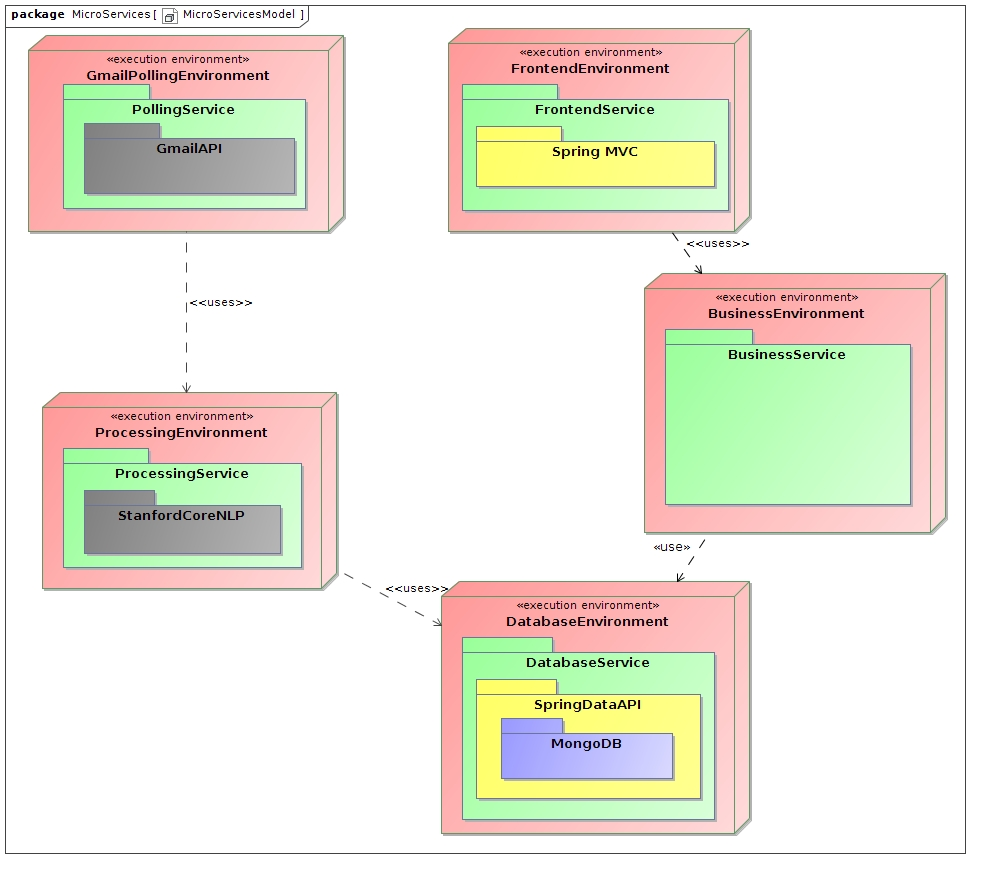
\includegraphics[width=\linewidth]{MicroServicesModel.jpg}
				\caption{Micro Services System Architecture}
				\label{MicroServicesAchitecture}
			\end{figure}
			\paragraph\indent
			The system is also well suited for this architecture since there are several modules that will have to interact with each other, but each serve a separate and specific purpose.
			
		\subsection{Services}			
			\subsubsection{Polling Service}\label{PollingSection}
			\paragraph\indent
			Figure \ref{PollingServiceModelFigure} shows the class diagram of the poller. A poller will either use long polling or polling with a sleep period afterwards (depending on what the API allows) to request new data from a specific PIM. Once it receives this information it will parse this information into a RawData object and add it into a queue which will be further processed by worker threads (see section  \ref{ProcessingServiceSection}).			
						
			\begin{figure}[!h]
			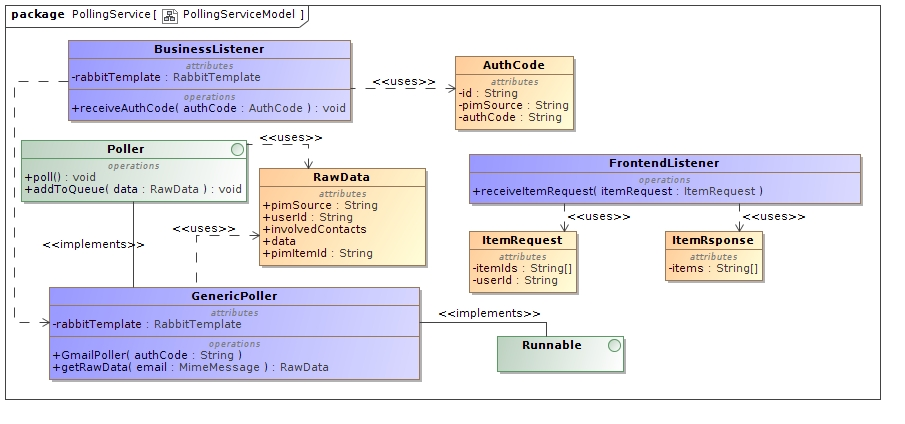
\includegraphics[width=\linewidth]{PollingServiceModel.jpg}
			\caption{Polling service.}
			\label{PollingServiceModelFigure}
			\end{figure}
			
						
			\subsubsection{Processing Service}\label{ProcessingServiceSection}
			\paragraph\indent
			Figure \ref{ProcessingModelFigure} shows the class diagram of the processing of raw data. Once raw data has been added to a queue by the poller in section \ref{PollingSection}, one of several worker threads will dequeue this raw data and pass the data to a Natural Language Processor (NLP). Once the NLP has finished processing the data the worker thread will parse this data into a ProcessedData object which will be sent to the database for persistence (see section \ref{DatabaseServiceSection}).
			
			\begin{figure}[!h]
			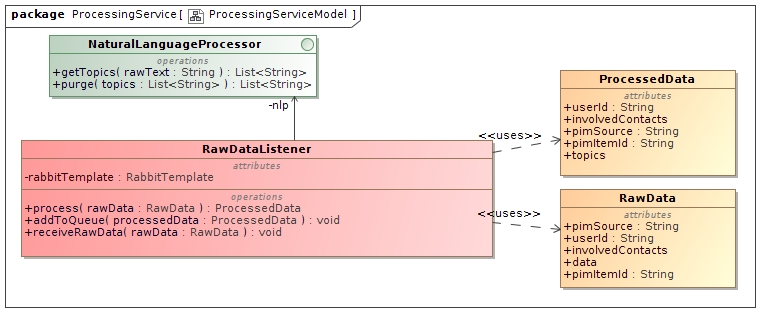
\includegraphics[width=\linewidth]{DataProcessingServiceModel.jpg}
			\caption{Processing service.}
			\label{ProcessingModelFigure}
			\end{figure}
						
			\subsubsection{Business Service} \label{BusinessServiceSection}
			Figure \ref{BsuinessServiceModelFigure} shows the class diagram of the business service. This service will start and stop polling services as users sign up/deactivate their accounts. Its purpose is basically to manage the other services based on user actions.

			\begin{figure}[!h]
				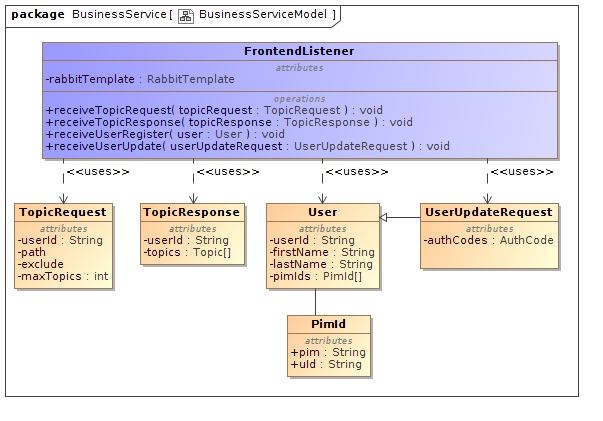
\includegraphics[width=\linewidth]{BusinessServiceModel.jpg}
				\caption{Business service.}
				\label{BsuinessServiceModelFigure}
			\end{figure}

			\subsubsection{Database Service} \label{DatabaseServiceSection}
			\paragraph\indent
			Figure \ref{DatabaseServiceModelFigure} shows the class diagram of the interface that will be used to communicate with the persistence API.			
						
			\begin{figure}[!h]
				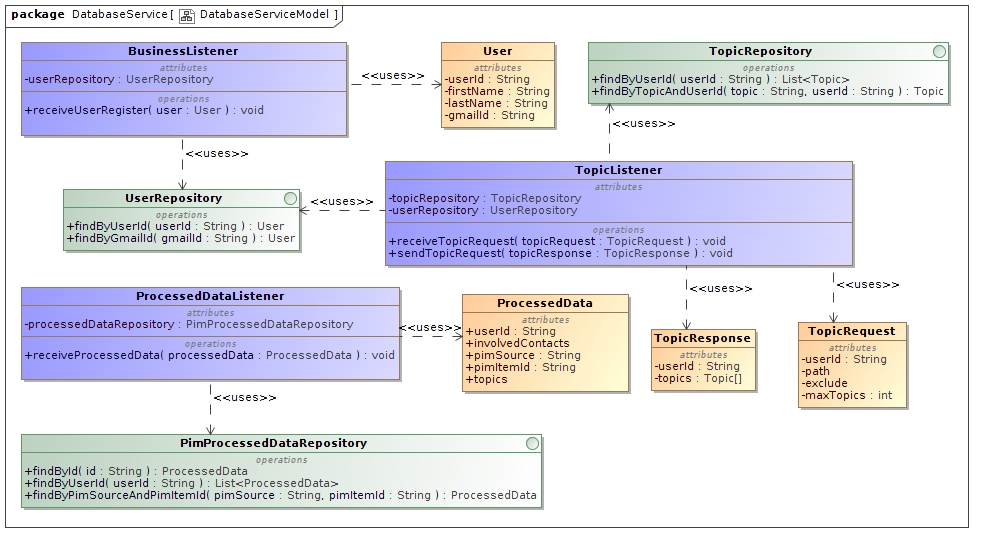
\includegraphics[width=\linewidth]{DatabaseServiceModel.jpg}
				\caption{Database service.}
				\label{DatabaseServiceModelFigure}
			\end{figure}
			
			\begin{figure}[!h]
				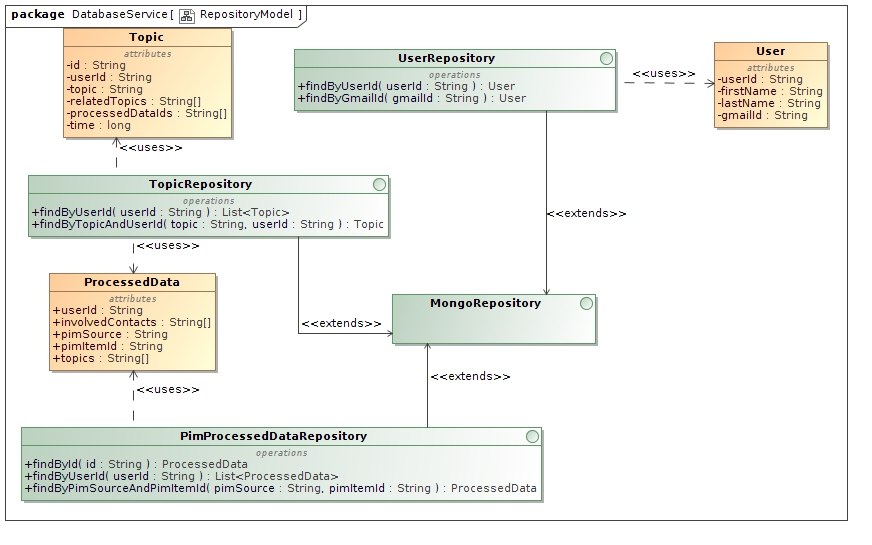
\includegraphics[width=\linewidth]{RepositoryModel.jpg}
				\caption{Repository Model.}
				\label{RepositoryModelFigure}
			\end{figure}
		
		\subsection{Tactics}
			\subsubsection{Flexibility}
				\begin{itemize}
					\item Hot reload and hot refresh.
					\item Contract based programming, i.e. providing proper interfaces that allows future expansion.
				\end{itemize}
			
			\subsubsection{Reliability}
				\begin{itemize}
					\item Ability to roll back database changes should an error occur during the change.
					\item Ability to restart services that have crashed due to some error that occurred.
				\end{itemize}
							
			\subsubsection{Security}
				\begin{itemize}
					\item Authentication will be required for a user to use the system.
					\item Data confidentiality will be achieved by using secure communication (HTTPS) and by applying salted hashing algorithms to keep passwords safe. Encryption will also be used on data that needs to be retrieved but has to be kept secure.
				\end{itemize}
		
	\section{Database and Persistence}
		\paragraph\indent
		We plan on using MongoDB as our database. This choice was made on the basis that a NoSQL database's document structure would fit our application's needs better than a standard relational database. MongoDB is also the perfect tool to use when data mining and high read and write loads are bought into play.
	
	\section{Process Specification}
		\paragraph\indent
		In this section we will address the manner in which the system will be implemented on a very abstract and overview manner.
		
		\subsection{Server}
			\paragraph\indent
			In the back end, the system would have a polling service that polls the PIMs for new information about the users. If a polling thread receives new data from the platform, they add this new data to a queue to be processed. Several worker threads dequeue data from the queue and uses natural language processing to determine the topic(s) contained in the data. This data is then added to a database and the corresponding topic(s) as well. When a user requests their bubble map, the system responds with all relevant topics of their life based on frequency and recency. The topics thus have a weight related to them that is calculated by the frequency and the temperal component. The weight is used to decide which topics should be selected. These topics are then returned to the user in the form of JSON objects. Once a user expands one of the bubbles a request is sent to the server to retrieve all the relevant topic corresponding to the topic to the user. These new topics is then added to the bubble map in the form of bubbles. Relevant topics are found on the basis of your own events and the events of your friends.
		
		\subsection{Front End}
			\paragraph\indent
			The user starts out with a root bubble that has relevant topics connected to it including a contacts bubble. All these bubbles can be expanded and reveal information related to that topic. The "contacts" bubble shows contacts you recently communicated with or might want to communicate with now. Other topics will expand into related topics and those can be expanded again and so forth. Upon expanding a topic a user can then interact with a specific occurrence in that topic (comment/reply) in a side panel that will be presented on the right of the screen.
	
	\section{Functional Requirements}		
		The following sections contain a brief overview of some of the functionality that will be provided by our system. The sections will become more detailed as development progresses.
		\subsection{Use Case Prioritisation}
			\textbf{Critical} (See figure \ref{UseCaseUserManagement})
			\begin{itemize}
			    \item Sign up
			    \item Choose PIMs
			    \item Login to PIMs
			    \item Logout
			    \item Expand bubble
			   	\item Display Data
			    \item Remove bubble
			\end{itemize}
		    
		    \textbf{Important} 
			\begin{itemize}
			    \item Deactivate Account
			    \item Reply to an email
			    \item Gain access to Gmail via our application
			    \item Set default depth factor
			    \item Set default branch factor
			\end{itemize}
		    
			
			\textbf{Nice-to-Have}
			\begin{itemize}
			    \item Set quick access depth factor
			    \item Set quick access branch factor
				\item Reset graph
				\item Customise colour scheme of interface
			    \item Help centre
			\end{itemize}
			
		
		\subsection{Use Case/Service Contracts}
			\subsubsection{Sign up}
				\textbf{Description:}  A user is required to sign up on our system. This entails using one's Google or Facebook account.\\
    			\textbf{Prioritisation:} Critical\\
      			\textbf{Pre-conditions}
    			\begin{itemize}
        			\item A user must have a Google or Facebook account.
        			\item The user must enter the correct information in order for the validation to be successful.
    			\end{itemize}
    			\textbf{Post-conditions}
     			\begin{itemize}
        			\item The user will have access to the functionality provided by our system.
        			\item The user may set their preferences as they wish.
        			\item The user may add or remove PIMs.
        			\item The user may log out of the system when they wish to.
        			\item The user may deactivate/delete their account should they so wish.
    			\end{itemize}
    			
    			\begin{figure}[!h]
    			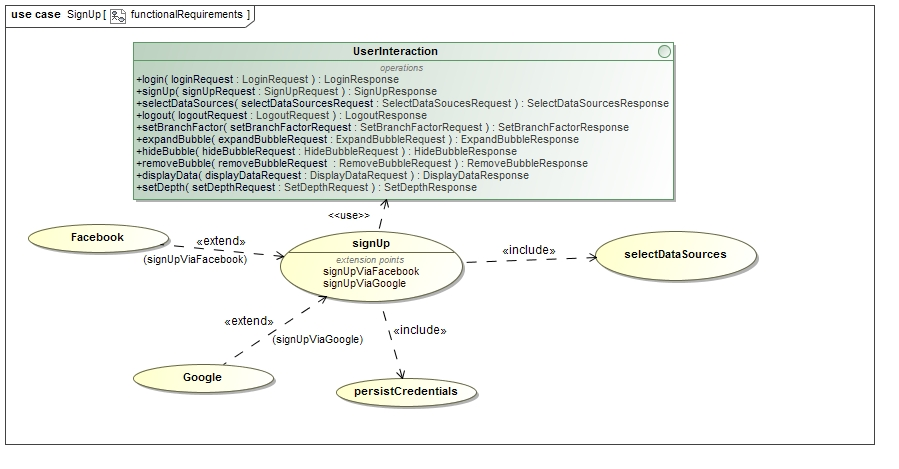
\includegraphics[width=\linewidth]{functionalRequirementsSignUp.jpg}
    			\caption{Use case diagram for Signing up}
    			\label{UseCaseSignUp}
    			\end{figure}
    			
    			\begin{figure}[!h]
    			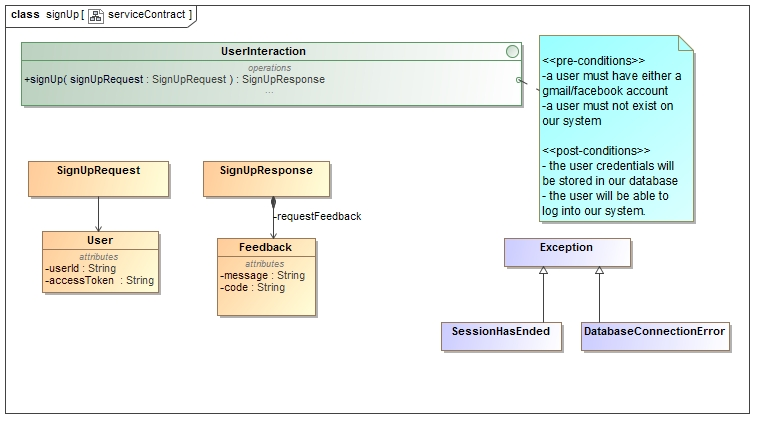
\includegraphics[width=\linewidth]{serviceContractSignUp.jpg}
    			\caption{Service contract diagram for Signing up}
    			\label{ServiceContractSignUp}
    			\end{figure}
    			
    		\subsubsection{Choose PIMs}
				\textbf{Description:}  A user is required to select the various PIMs they wish to be used when extracting data to build their bubble map.\\
    			\textbf{Prioritisation:} Critical\\
      			\textbf{Pre-conditions}
    			\begin{itemize}
        			\item A user must be registered.
        			\item A user must be logged in to the system.
        			\item The user must have an active and valid account for that specific PIM.
    			\end{itemize}
    			\textbf{Post-conditions}
     			\begin{itemize}
        			\item The user may add or remove PIMs.
        			\item The selected PIMs will be mined for data.
        			\item The unselected PIMs will not be mined for data.
    			\end{itemize}

    			\begin{figure}[!h]
    			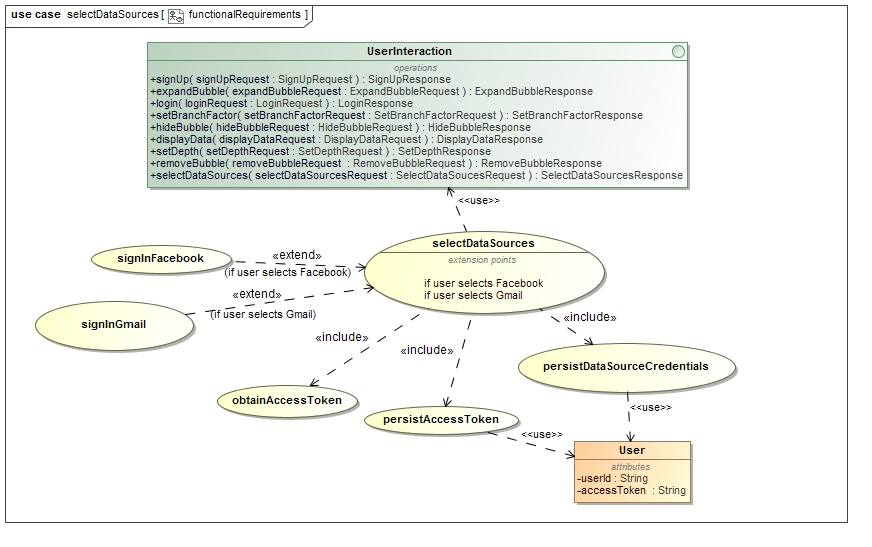
\includegraphics[width=\linewidth]{functionalRequirementsSelectDataSources.jpg}
    			\caption{Use case diagram for selecting data sources}
    			\label{UseCaseSelectDataSources}
    			\end{figure}
    			
    			\begin{figure}[!h]
    			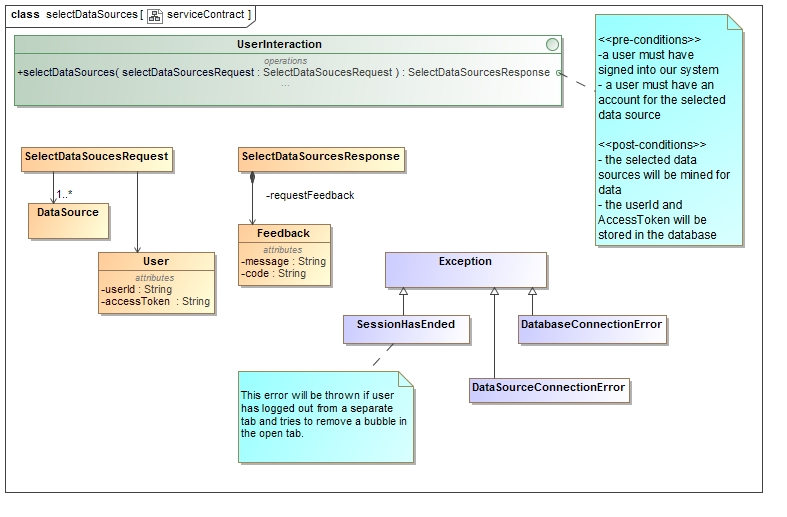
\includegraphics[width=\linewidth]{serviceContractSelectDataSources.jpg}
    			\caption{Service contract diagram for selecting data sources}
    			\label{ServiceContractSelectDataSources}
    			\end{figure}
    			
    			
    			
    		\subsubsection{Login to PIMs}
				\textbf{Description:}  A user will login with their Google account. This will be done by using the OAUTH protocol which is compatible with the Google and Facebook API.\\
    			\textbf{Prioritisation:} Critical\\
      			\textbf{Pre-conditions}
    			\begin{itemize}
        			\item A user must be logged in to the system.
        			\item A user must have selected at least one PIM.
        			\item A user must have an active and valid account for that PIM.
    			\end{itemize}
    			\textbf{Post-conditions}
     			\begin{itemize}
        			\item The PIMs will be mined for data.
        			\item The login credentials for that PIM for a specific user will be stored in our database.
    			\end{itemize}
    			
    			\begin{figure}[!h]
    			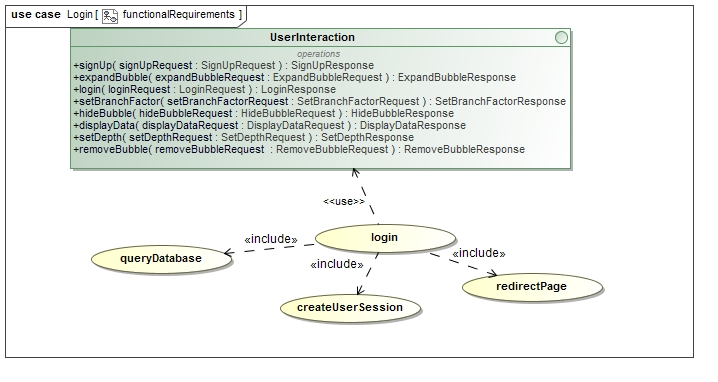
\includegraphics[width=\linewidth]{functionalRequirementsLogin.jpg}
    			\caption{Use case diagram for Logging in}
    			\label{UseCaseLogin}
    			\end{figure}
    			
    			\begin{figure}[!h]
    			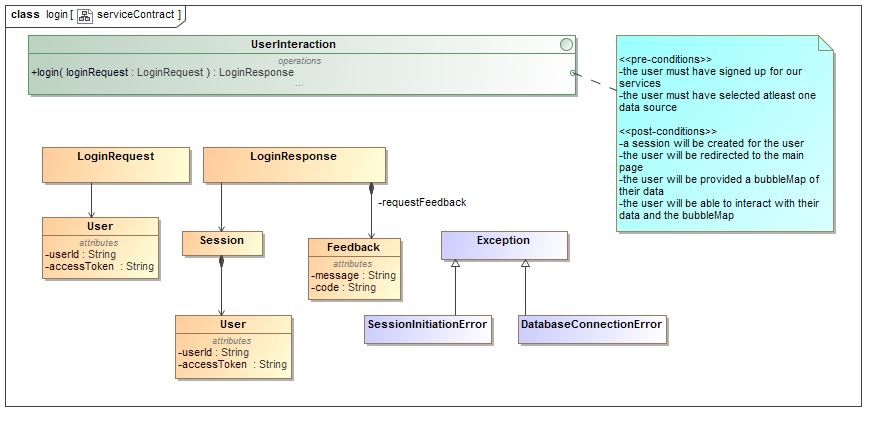
\includegraphics[width=\linewidth]{serviceContractLogin.jpg}
    			\caption{Service contract diagram for Logging in}
    			\label{ServiceContractLogin}
    			\end{figure}
    			
    		\subsubsection{Logout}
				\textbf{Description:}  A user can choose to log out of the system in a secure manner.\\
    			\textbf{Prioritisation:} Critical\\
      			\textbf{Pre-conditions}
    			\begin{itemize}
        			\item A user must be registered on the system and logged in to the system.
    			\end{itemize}
    			\textbf{Post-conditions}
     			\begin{itemize}
        			\item The user will not have access to the main functionality provided by the system.
        			\item The user will need to log in again to access their bubble map.
    			\end{itemize}

    		\begin{figure}[!h]
    			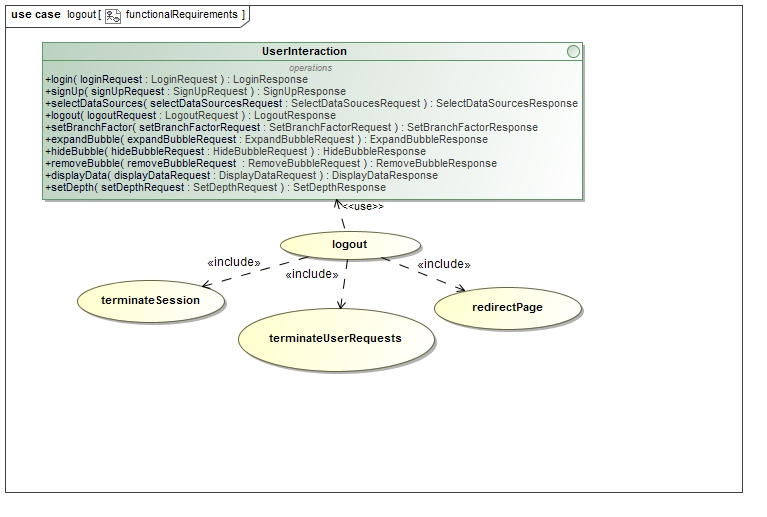
\includegraphics[width=\linewidth]{functionalRequirementsLogout.jpg}
    			\caption{Use case diagram for Logging out}
    			\label{UseCaseLogout}
    			\end{figure}
    			
    			\begin{figure}[!h]
    			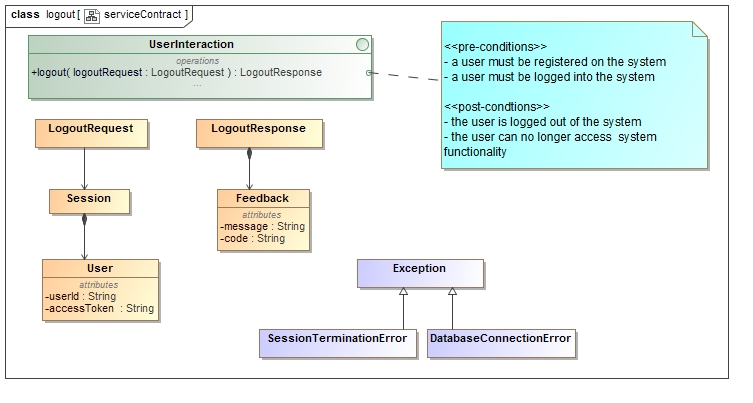
\includegraphics[width=\linewidth]{serviceContractLogout.jpg}
    			\caption{Service contract diagram for Logging out}
    			\label{ServiceContractLogout}
    			\end{figure}
    			
    		\subsubsection{Expand Bubble}
				\textbf{Description:}  A user can choose to expand a bubble to reveal more topics related to the bubble.\\
			    \textbf{Prioritisation:} Critical\\
      			\textbf{Pre-conditions}
			    \begin{itemize}
			        \item A user must be registered and logged in on the system.
			        \item A user must have selected one or more PIMs to be mined.
			    \end{itemize}
			    \textbf{Post-conditions}
			     \begin{itemize}
			        \item The system will expand the bubble Map and introduce new topics.
			    \end{itemize}
			    
			    \begin{figure}[!h]
    			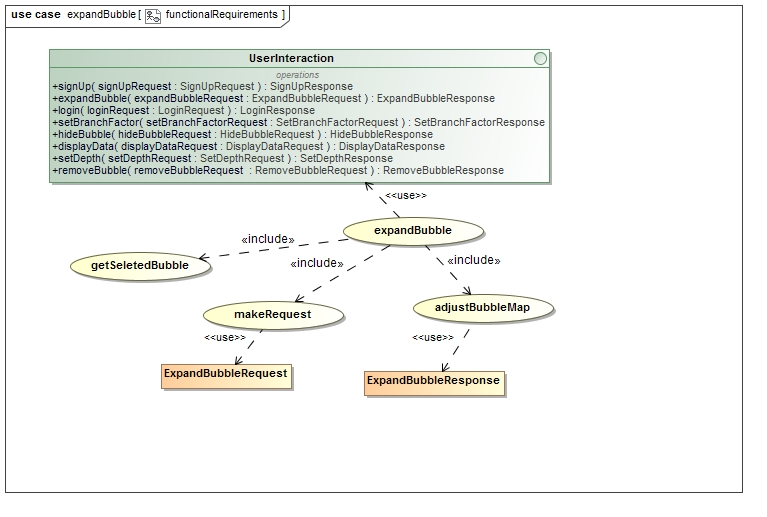
\includegraphics[width=\linewidth]{functionalRequirementsExpandBubble.jpg}
    			\caption{Use case diagram for Expanding a Bubble}
    			\label{UseCaseExpandBubble}
    			\end{figure}
    			
    			\begin{figure}[!h]
    			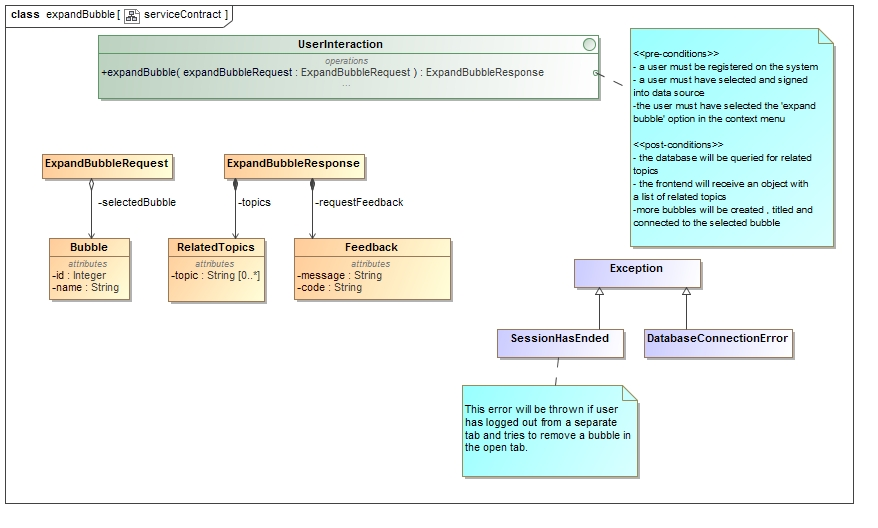
\includegraphics[width=\linewidth]{serviceContractExpandBubble.jpg}
    			\caption{Service contract diagram for Expanding a Bubble}
    			\label{ServiceContractExpandBubble}
    			\end{figure}
			    
    		\subsubsection{Display Data}
				\textbf{Description:}  A user can choose to view a bubble to reveal specific data and functionality surrounding a chosen bubble.\\
			    \textbf{Prioritisation:} Critical\\
			    \textbf{Pre-conditions}
			    \begin{itemize}
			        \item A user must be registered and logged in on the system.
			        \item A user must have selected PIMs to be mined.
			    \end{itemize}
				\textbf{Post-conditions}
				\begin{itemize}
					\item The system will reveal specific data regarding this topic in a side panel.
					\item The system will provide certain functionality for certain types of data e.g. a Facebook post will have the functionality to be like, commented on or shared.
				\end{itemize}
				
			\begin{figure}[!h]
    			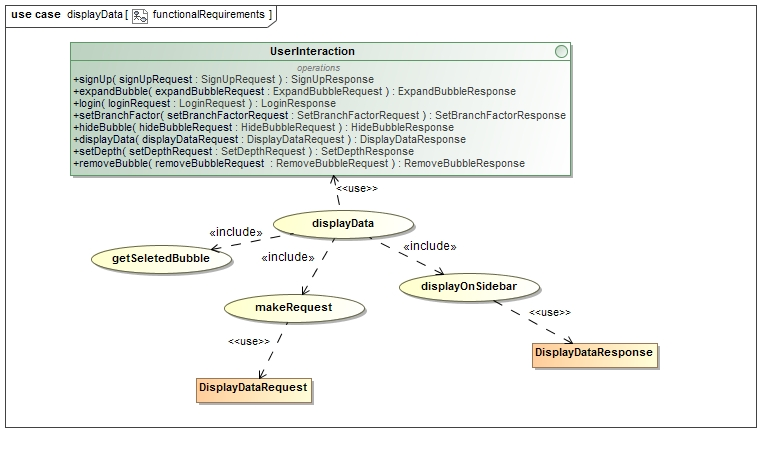
\includegraphics[width=\linewidth]{functionalRequirementsDisplayData.jpg}
    			\caption{Use case diagram for Displaying data}
    			\label{UseCaseDisplayData}
    			\end{figure}
    			
    			\begin{figure}[!h]
    			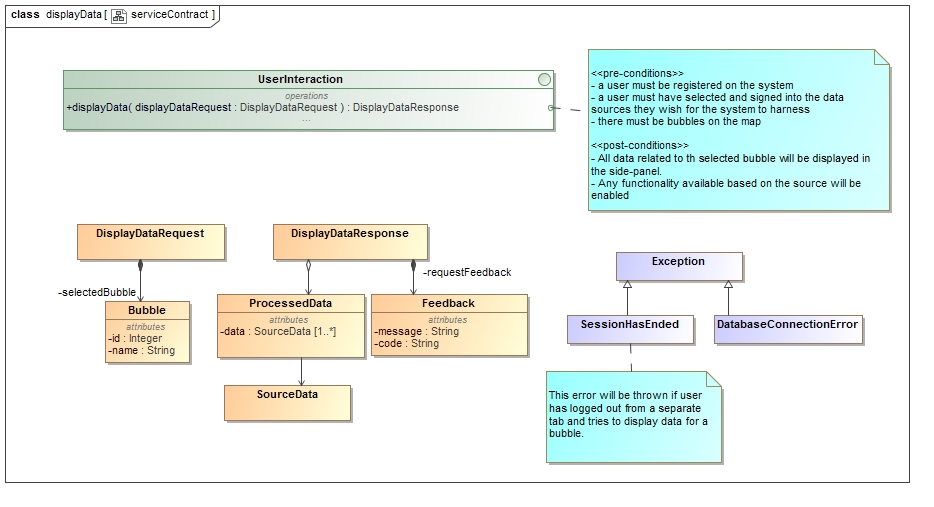
\includegraphics[width=\linewidth]{serviceContractDisplayData.jpg}
    			\caption{Service contract diagram for Displaying data}
    			\label{ServiceContractDisplayData}
    			\end{figure}
				
    		\subsubsection{Remove Bubble}
				\textbf{Description:}  A user can choose to remove a bubble which will remove all bubbles related to it.\\
			    \textbf{Prioritisation:}Critical\\
     			\textbf{Pre-conditions}
				\begin{itemize}
					\item A user must be registered and logged in on the system.
					\item A user must have selected PIMs to be mined.
				\end{itemize}
    			\textbf{Post-conditions}
     			\begin{itemize}
			        \item The system will remove the specified bubble.
			        \item The system will remove all bubbles in the sub branch of the selected bubble.
    			\end{itemize}
    			
    			\begin{figure}[!h]
    			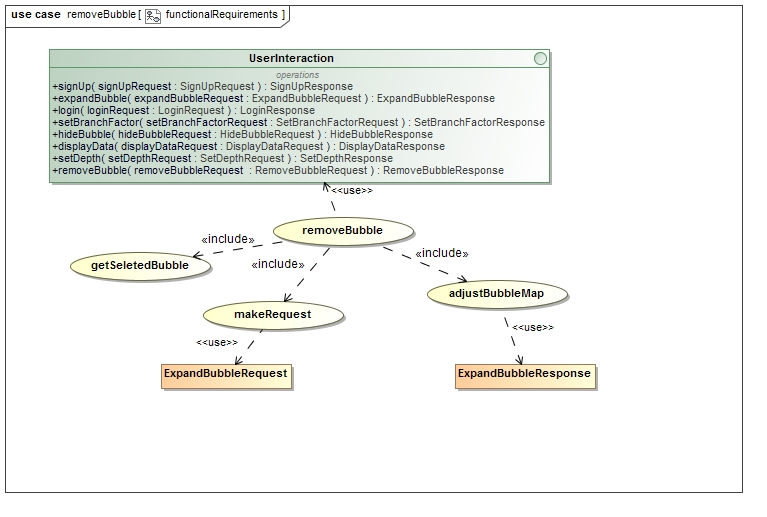
\includegraphics[width=\linewidth]{functionalRequirementsRemoveBubble.jpg}
    			\caption{Use case diagram for removing a bubble}
    			\label{UseCaseRmoveBubble}
    			\end{figure}
    			
    			\begin{figure}[!h]
    			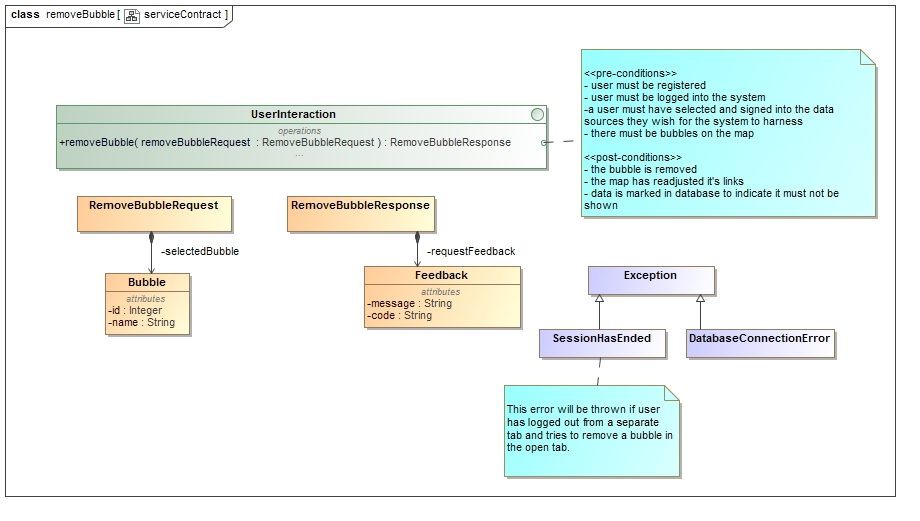
\includegraphics[width=\linewidth]{serviceContractRemoveBubble.jpg}
    			\caption{Service contract diagram for removing a bubble}
    			\label{ServiceContractRemoveBubble}
    			\end{figure}
    		
    		%___________________IMPORTANT_____________________
    		
    		\subsubsection{Deactivate Account}
				\textbf{Description:}  A user can choose to permanently delete their account or deactivate it.\\
    			\textbf{Prioritisation:} Important\\
      			\textbf{Pre-conditions}
    			\begin{itemize}
        			\item A user must be registered on the system.
    			\end{itemize}
    			\textbf{Post-conditions}
     			\begin{itemize}
        			\item The user will not have access to the main functionality provided by the system.
        			\item The user will need to sign up again to access the system functionality.
    			\end{itemize}
    			
			    
    		\subsubsection{Specify the default depth factor}
				\textbf{Description:}  A user can choose the number of levels the bubble map should expand when they open the map for the first time during the current session.\\
			    \textbf{Prioritisation:} Important\\
      			\textbf{Pre-conditions}
			    \begin{itemize}
			        \item A user must be registered and logged in on the system.
			        \item A user must have selected PIMs to be mined.
			    \end{itemize}
    			\textbf{Post-conditions}
     			\begin{itemize}
        			\item The user's bubble map will modify itself to adapt to the user's specifications.
    			\end{itemize}
    			
    			\begin{figure}[!h]
    			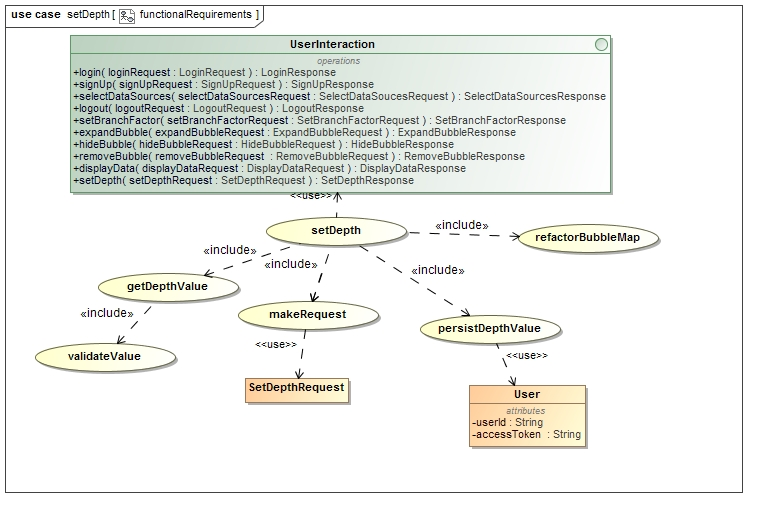
\includegraphics[width=\linewidth]{functionalRequirementsSetDepth.jpg}
    			\caption{Use case diagram for setting default depth}
    			\label{UseCaseSetDepth}
    			\end{figure}
    			
    			\begin{figure}[!h]
    			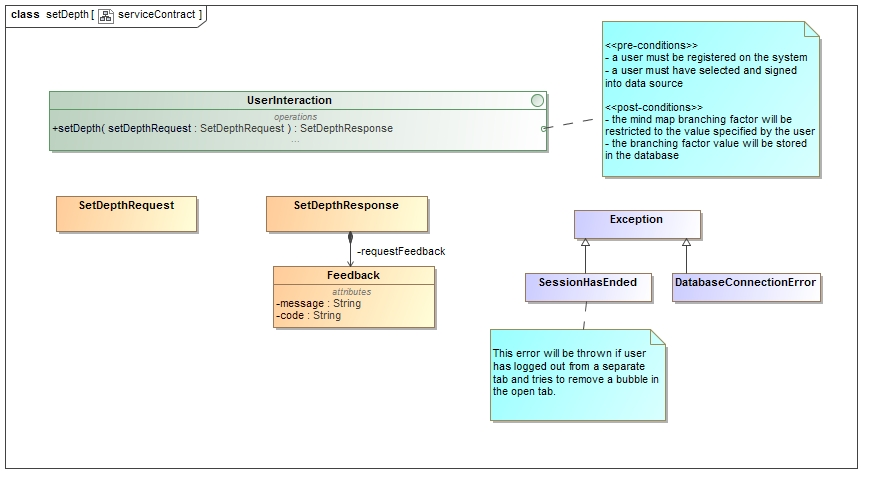
\includegraphics[width=\linewidth]{serviceContractSetDepth.jpg}
    			\caption{Service contract diagram for setting default depth}
    			\label{ServiceContractSetDepth}
    			\end{figure}
    			
    		\subsubsection{Specify the default branch factor}
				\textbf{Description:}  A user can choose specify how many branches the bubble map will initially have.\\
			    \textbf{Prioritisation:} Important\\
      			\textbf{Pre-conditions}
			    \begin{itemize}
			        \item A user must be registered and logged in on the system.
			        \item A user must have selected PIMs to be mined.
			    \end{itemize}
    			\textbf{Post-conditions}
			    \begin{itemize}
			    	\item The user's bubble map will modify itself to adapt to the user's specifications.
    			\end{itemize}
    			
    			\begin{figure}[!h]
    			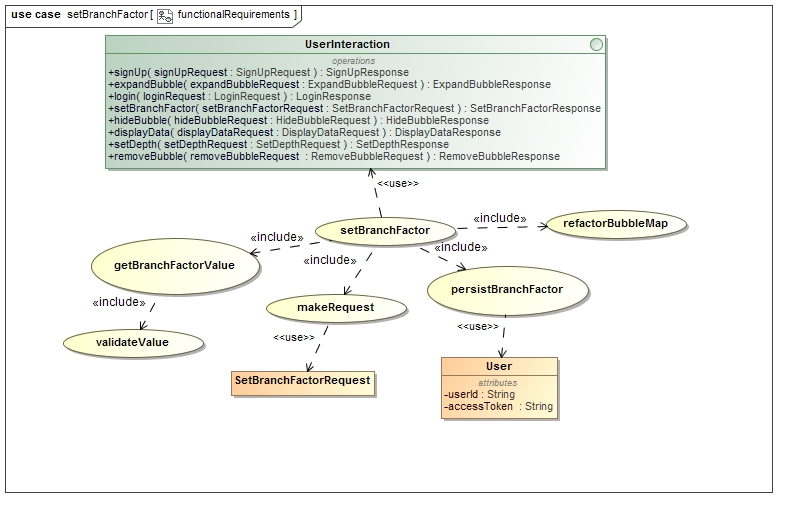
\includegraphics[width=\linewidth]{functionalRequirementsSetBranchFactor.jpg}
    			\caption{Use case diagram for setting default branch factor}
    			\label{UseCaseDisplayData}
    			\end{figure}
    			
    			\begin{figure}[!h]
    			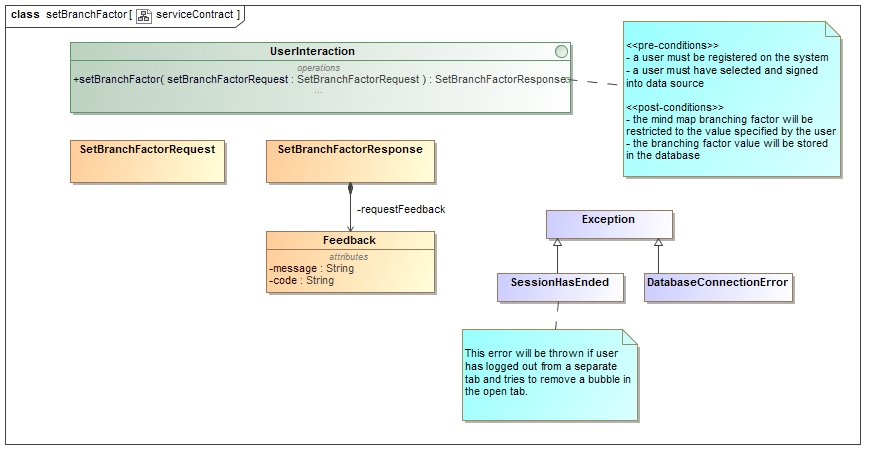
\includegraphics[width=\linewidth]{serviceContractSetBranchFactor.jpg}
    			\caption{Service contract diagram for setting default branch factor}
    			\label{ServiceContractDisplayData}
    			\end{figure}
    			
    		\subsubsection{Reply to an email}
				\textbf{Description:}  A user can respond to an email directly from our application\\
			    \textbf{Prioritisation:} Important\\
      			\textbf{Pre-conditions}
			    \begin{itemize}
			        \item A user must be registered and logged in on the system.
			        \item A user must have selected an email source.
			    \end{itemize}
    			\textbf{Post-conditions}
			    \begin{itemize}
			    	\item The user will be able to reply to a message that has been displayed by our system
    			\end{itemize}
    			
    		\subsubsection{Redirect to Gmail application from our application}
				\textbf{Description:}  A user can respond to an email directly from our application\\
			    \textbf{Prioritisation:} Important\\
      			\textbf{Pre-conditions}
			    \begin{itemize}
			        \item A user must be registered and logged in on the system.
			        \item A user must have selected an email source.
			    \end{itemize}
    			\textbf{Post-conditions}
			    \begin{itemize}
			    	\item The user will be able to navigate to Gmail from our application
    			\end{itemize}
    			
    		%_________________________Nice-to-Have____________________
    	    
    	    \subsubsection{Set quick access depth factor}
				\textbf{Description:}  Manipulate the BubbleMap quickly but not affect its state permanently\\
			    \textbf{Prioritisation:} Nice-to-Have\\
      			\textbf{Pre-conditions}
			    \begin{itemize}
			        \item A user must be registered and logged in on the system.
			    \end{itemize}
    			\textbf{Post-conditions}
			    \begin{itemize}
			    	\item The user will be able to change BubbleMap depth factor for instant manipulation
    			\end{itemize}
    		
    		\subsubsection{Set quick access branch factor}
				\textbf{Description:}  Manipulate the BubbleMap quickly but not affect its state permanently\\
			    \textbf{Prioritisation:} Nice-to-Have\\
      			\textbf{Pre-conditions}
			    \begin{itemize}
			        \item A user must be registered and logged in on the system.
			    \end{itemize}
    			\textbf{Post-conditions}
			    \begin{itemize}
			    	\item The user will be able to change BubbleMap branch factor for instant manipulation
    			\end{itemize}
    		
    		\subsubsection{Reset graph}
				\textbf{Description:} Reset the graph to the state it was in when it loaded that session\\
			    \textbf{Prioritisation:} Nice-to-Have\\
      			\textbf{Pre-conditions}
			    \begin{itemize}
			        \item A user must be registered and logged in on the system.
			    \end{itemize}
    			\textbf{Post-conditions}
			    \begin{itemize}
			    	\item The user will be able to revert all changes to the BubbleMap settings
    			\end{itemize}
    			
    	    \subsubsection{Customise colour scheme}
				\textbf{Description:} Change the colour scheme of the interface\\
			    \textbf{Prioritisation:} Nice-to-Have\\
      			\textbf{Pre-conditions}
			    \begin{itemize}
			        \item A user must be registered and logged in on the system.
			    \end{itemize}
    			\textbf{Post-conditions}
			    \begin{itemize}
			    	\item The user will be able to change the BubbleMap background colour
			    	\item The user will be able to change the Navigation bar colour
			    	\item The user will be able to change the sidepanel colour
    			\end{itemize}
    			
    		\subsubsection{Help Centre}
				\textbf{Description:} A means of communication between users and the developers\\
			    \textbf{Prioritisation:} Nice-to-Have\\
      			\textbf{Pre-conditions}
			    \begin{itemize}
			        \item A user must be registered and logged in on the system.
			    \end{itemize}
    			\textbf{Post-conditions}
			    \begin{itemize}
			    	\item The user will be able to contact the developers and report issues or ask for assistance if the Help/FAQ page did not suffice 
    			\end{itemize}
    			
		\subsection{Required Functionality}
			Functionality that should be included in the system includes:
			\begin{itemize}
				\item A login/sign up system. 
				\item Adding various PIMs to your account.
				\item Interaction with PIMs directly from the bubble map itself (commenting, emailing, etc.).
				\item Expanding bubbles in order to find articles related to that bubble.
				\item Rapidly integrate new information into the system.
				\item Logs will be used to track any unhandled exceptions or problems.
			\end{itemize}
		\newpage
		\subsection{Domain Model}
		\begin{figure}[!h]
			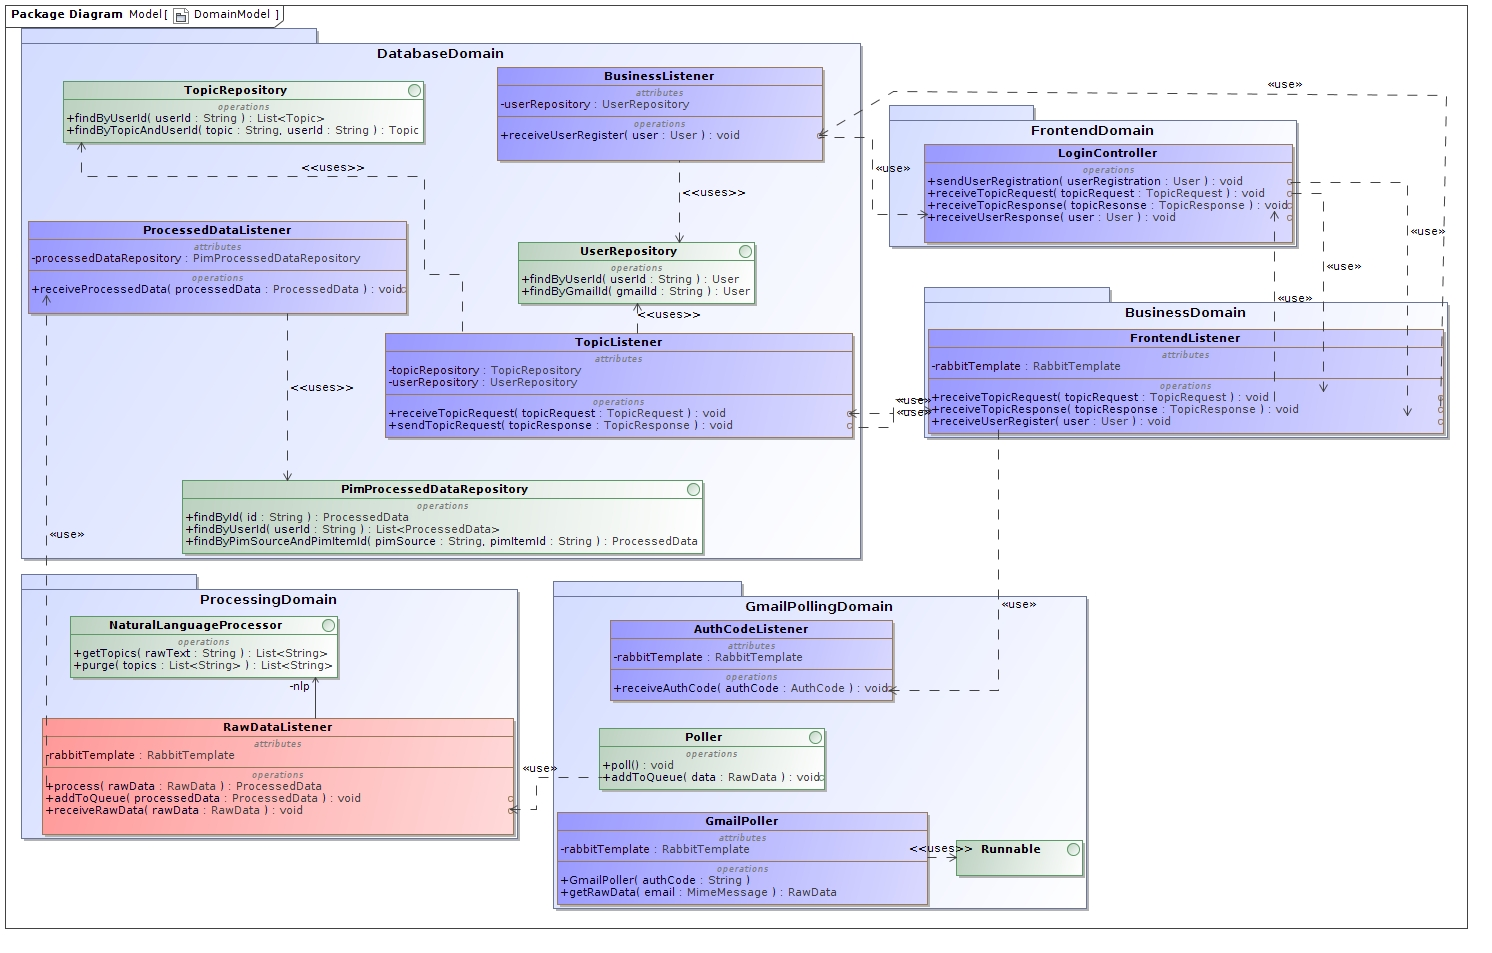
\includegraphics[width=\linewidth]{DomainModel.jpg}
			\caption{Class Diagram: Domain Model}
			\label{DomainModel}
		\end{figure}
		\paragraph\indent
		The mind map for a user will portray information from PIMs requested by the user. The mind map will consist of a root node containing child nodes of relevant information (topics). Each topic will point to a PIM (Facebook, Google etc.) and will contain a list of information relative to the topic.
			
	\section{Technologies}
		\subsection{Framework}
			\paragraph\indent
			The framework we decided to use is Spring Boot. This was chosen on the fact that Spring is a lot more lightweight than JavaEE. Spring also uses the convention-over-configuration idea that simplifies the learning experience.
			
			\paragraph\indent
			Spring is a well known framework with a large community of support. It is highly scalable and works towards being stateless. Spring also integrates well with technologies like Tomcat and build tools like Gradle. Spring Boot was chosen over Spring MVC for its simplicity.
			
			\paragraph\indent
			Research on Google's framework "Google Guice" was also done as an alternative, and while it is a good architecture in terms of what it does and how it makes it simpler for the programmer by moving away from XML, it is still a relatively new framework and does not have much support yet. Spring has been tried and tested and the fault tolerance on Spring is the deciding factor over Google Guice.
			
		\subsection{Web Container}
			\paragraph\indent
			The web container we have chosen to use is Tomcat. Since, as mentioned before, we have chosen to use Spring as our framework Tomcat would be the obvious choice, given it has good integrability with Spring.
			
			\paragraph\indent
			Jetty was also considered but due to the amount of documentation and experience that Tomcat has over Jetty, the choice was made to rather go with Tomcat. Benchmark tests were also run with Tomcat, Jetty, Glassfish and it was shown that Tomcat was the better contender.
			
			\paragraph\indent
			We have decided to move away EJB containers and thus JavaEE containers to use the much lighter web container server in response to the dynamics of our particular system which required a fast, light footprint system to run our framework on.
		
		\subsection{Natural Language Processor}
			\paragraph\indent
			Due to the complexities involved in getting Google's Parsey McParseFace set up, the Stanford CoreNLP will be used to analyse the syntax and underlying topics of sentences.
			
		\subsection{Build Tool}
			\paragraph\indent
			Gradle was chosen as the build tool due to its simplicity and simplistic integrability with Spring. It also doesn't use the XML approach that Maven uses but rather uses a more natural programming style that is recognizable.
			
		\subsection{Communication}
			\paragraph\indent
			WebSockets will be used to have a persistent client to server communication that will create a low latency, real time interaction, a requirement for our system. Some of the advantages of WebSockets is its high scalability, high performance and protocol layering.
			
			\paragraph\indent
			A hypothesis with WebSockets initially was that not all browsers could support this technology. This was however proven incorrect as tests ran on all browsers showed that every browser except Opera mini (A mobile client for Opera) supported WebSockets. \sloppy\url{http://caniuse.com/\#feat=websockets}
	\section{Initial Design}

    	\begin{figure}[!h]
			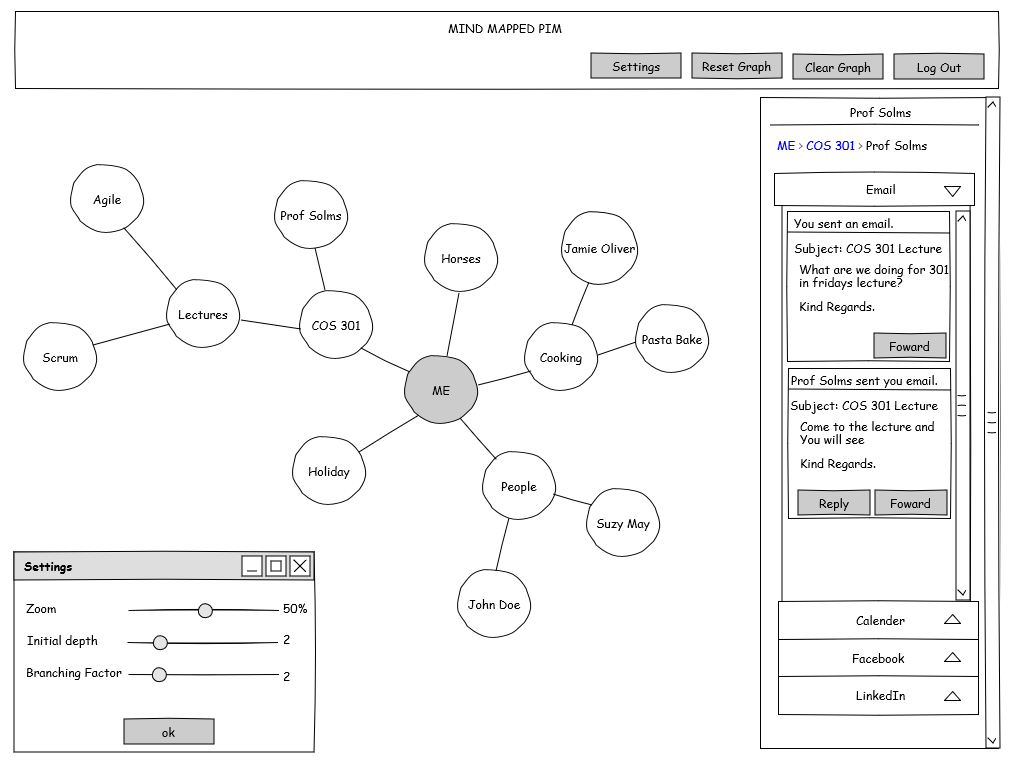
\includegraphics[width=\linewidth]{Main - Email Expanded.png}
			\caption{Main Interface- Email Expanded}
			\label{Main}
		\end{figure}
		\paragraph\indent
		An initial Idea for the main mind map interface, drawn with wire frames, with a sidebar that shown the currently active node "Prof Solms" with relevant information on why and what information is relevant. In this figure the Emails column is expanded, in the next figure the Calender will be expanded.
    	\begin{figure}[!h]
    		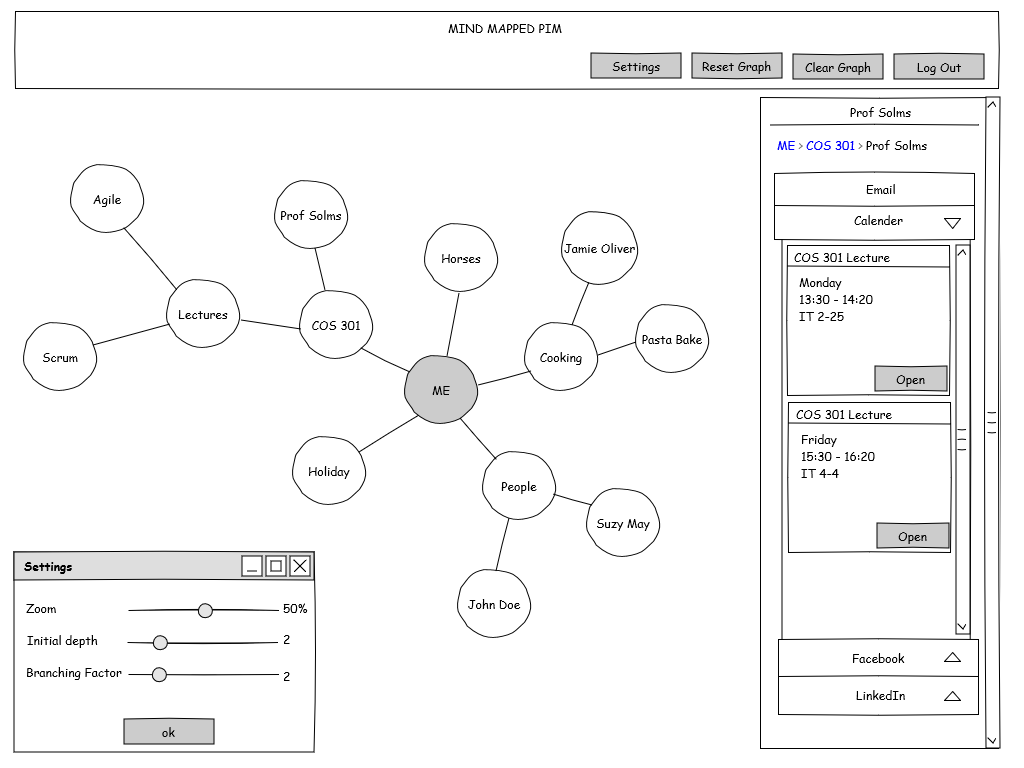
\includegraphics[width=\linewidth]{Main - Calender Expanded.png}
    		\caption{Main Interface- Calender Expanded}
    		\label{Main}
    	\end{figure}

	\section{Open Issues}
		\begin{itemize}
			\item What we are going to use for our physical server?
			\item How often should the mind map refresh?
			\item How much data mining should be done before the information is displayed and the mining starts being done behind the scenes?
			\item Should removing bubbles remove data from the database or not?
			\item Is a privacy policy required?
		\end{itemize}
\end{document}
